\chapter{Проектирование архитектуры приложения}
Для создания MVP системы достаточно создать SPA-приложение, которые вместит в себя весь необходимый функционал.
Его архитектура имеет свледующий вид:
\begin{itemize}
	\item \textbf{Front-end} часть, отвечающая за отрисовку данных. Она должна включать: интерактивную карту, с возвожностью построения точек и полигонов, хранилище построенных объектов, перечень функций для обработки и визуализации данных первой очереди, а также поиск по городам.
	\item \textbf{Back-end} часть отвечает за связь с распределенными базами данных, описанными в предыдущей главе и выступает, своего рода, прокси сервисом, который формирует запросы к специализированным системам.
\end{itemize}

Связь между частями осуществляется с помощью JSON API. Кроме того, расположение на единой хостовой машине, сводит задержку передачи данных до минимума (рис. \ref{fig:archecture}).

\begin{figure}[h]  % Окружение для картинки
	\centering
	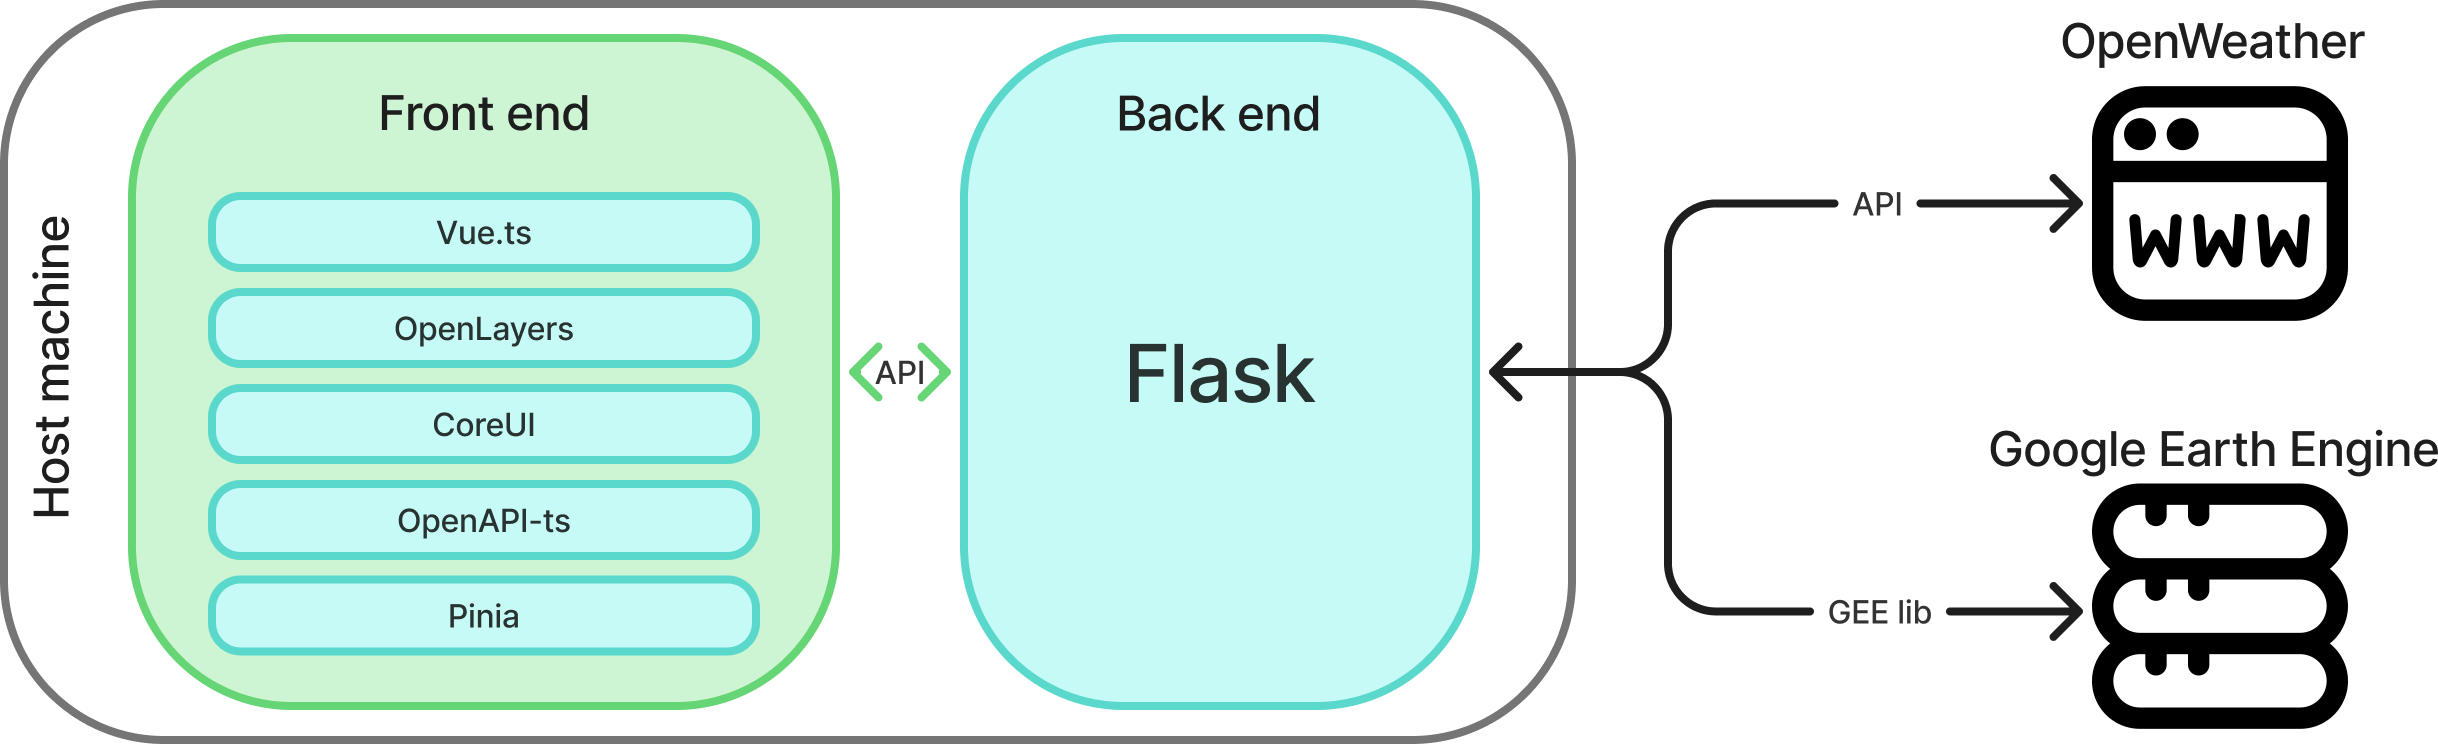
\includegraphics[height=0.3\textwidth]{imgs/arch.png}  % Вставка изображения
	\caption{Архитектура приложения.}  % Подпись к изображению
	\label{fig:archecture}  % Метка для ссылки
\end{figure}
